% % % % % % % % % % % % % % 
% 
% Skript zu NUMERIK I
% WS14/15
% von Prof. Dr. Blank
% Universität Regensburg
% 
% 
%	Kap. 4: Lineare Gleichungssysteme: Direkte Methoden (Fortsetzung)
% 
% % % % % % % % % % % % % % 



\chapter{Lineare Gleichungssysteme: Direkte Methoden (Fortsetzung)}

\sectione{Gaußsches Eliminationsverfahren mit Aquilibrierung und Nachiteration}

Mit Skalierung $D_zA$ (\textbf{Zeilenskalierung})\index{Skalierung!Zeilen-} oder
$D_sA$ (\textbf{Spaltenskalierung})\index{Skalierung!Spalten-}
mittels Diagonalmatrizen $D_z, D_s$ 
lässt sich eine Pivotstrategie beliebig abändern.
Jetzt ist die Frage:

\textit{Was ist eine \enquote{gute} Skalierung?}

Skalierung ändert die Länge der Basisvektoren 
des Bild- bzw. des Urbildvektorraumes.
Durch Normierung der Länge auf 1 
wird die Pivotstrategie unabhängig von der gewählten Einheit.

Sei $A\in\Renm $ und $\nn $ eine Vektornorm.

\subsectione{Äquilibrierung der Zeilen} \index{Äquilibrierung!Zeilen-}
Alle Zeilen von $D_zA$ haben die gleiche Norm, z.B. $\nn =1$, wofür 
\begin{gather}
  D_z = \begin{pmatrix}
    \sigma_1 & & 0 \\
    &\ddots & \\ 
    0 && \sigma_n
  \end{pmatrix}
  \quad \text{ mit }\sigma_i\coloneqq \frac{1}{\nn[(a_{i1}, \dotsc , a_{im})]}
  \label{IV.1.1}
\end{gather}
gesetzt wird.


\subsectione{Äquilibrierung der Spalten} \index{Äquilibrierung!Spalten-}
Alle Spalten von $AD_s$ haben die gleiche Norm, z.B. $\nn =1$, wofür 
\begin{gather}
  D_s = \begin{pmatrix}
    \tau_1 & & 0 \\
    &\ddots & \\ 
    0 && \tau_m
  \end{pmatrix}
  \quad \text{ mit }\tau_j\coloneqq \nn[\begin{pmatrix}
    a_{1j} \\ \vdots \\ a_{nj}
  \end{pmatrix}]^{-1}
  \label{IV.1.2}
\end{gather}
gesetzt wird.

Äquilibrierung von Zeilen \textbf{und} Spalten 
führt zu einem nichtlinearen Gleichungssystem und ist i.d.R. aufwendig.


\begin{Leme}
  \label{4.3.1}
  Sei $A$ zeilenäquilibriert bzgl. der $l_1$-Norm, dann gilt:
  \begin{gather}
    cond_{\infty}(A) \leq cond_{\infty}(DA)  \label{IV.1.3}
  \end{gather}
  für alle regulären Diagonalmatrizen $D$.
\end{Leme} 

\begin{proof}
  siehe Übungsaufgabe
\end{proof}

Wie in Kapitel \ref{3} gesehen, kann die Näherungslösung $\tilde{x}$ 
trotz Pivotisierung und Äquilibrierung noch sehr ungenau sein.


\subsectione{Nachiteration} \index{Nachiteration}
Die Näherung $\tilde{x}$ kann durch Nachiteration verbessert werden.
Falls $\tilde{x}$ exakt ist, gilt:
\begin{gather}
  r(\tilde{x}) \coloneqq b-A\tilde{x} =0 \label{IV.1.4}
\end{gather}
ansonsten ist $A(x-\tilde{x})=r(\tilde{x}).$ \ \
Also löse die Korrekturgleichung
\begin{gather}
  A\Delta x = r(\tilde{x}) 	\label{IV.1.5}
\end{gather}
und setze $x^{(1)} \coloneqq \tilde{x} +\Delta x$
Wiederhole dies sooft, bis $x^{(i)}$ \enquote{genau genug} ist.
Die Lösung $\tilde{x}$ wird durch Nachiteration 
meist mit sehr gutem Erfolg verbessert
\cite[genaueres in ][]{dahmenreusken}.

\eqref{IV.1.5} wird mit der bereits vorhandenen LR-Zerlegung
nur mit der neuen rechten Seite $r(\tilde{x})$ gelöst, 
d.h. eine vorwärts und eine Rückwärtssubstitution
mit $\mathcal{O}(n^2)$ flops.


\begin{Beme}[nach Skeel 1980]
  Die Gauß-Elimination mit Spaltenpivotsuche und einer Nachiteration
  ist komponentenweise stabil.
\end{Beme}


\sectione{Cholesky-Verfahren}
Im Folgenden sei $A$ eine symmetrische, positiv definite Matrix in $\Renn $, d.h.
$A=A^T$ und $\langle x, Ax \rangle = x^TAx > 0$ für alle $ x\neq 0$. 
(kurs: \textbf{spd Matrix}) \index{spd Matrix}

\begin{Satze}
  \label{4.2.1}
  Für jede spd Matrix $A\in \Renn $ gilt:
  \begin{enumerate}[i)]	
  \item $A$ ist invertierbar
  \item $a_{ii}>0$ für $i=1, \dotsc , n$
  \item $\max_{ij}|a_{ij}| = \max_{i}a_{ii}$
  \item Bei der Gauß-Elimination ohne Pivotsuche 
    ist jede Restmatrix wieder eine spd Matrix.
  \end{enumerate}
\end{Satze}

\begin{proof}~
  \begin{enumerate}[i)]
  \item Es gilt $x^TAx\neq 0\Rightarrow Ax\neq 0$. 
    Nach ii) ist $Ax\neq 0~\forall x\in\Ren\backslash \{0\}$
    also $ker(A)=0$. %folgt aus \eqref{IV.2.1}
  \item Sei $e_i$ der $i$-te Einheitsvektor, so folgt $a_{ii} = e_{i}^TAe_i > 0$.
  \item siehe Übungsaufgabe
  \item Es gilt:
    \begin{align*}
      A^{(1)} 
      &\coloneqq A = \begin{pmatrix}
        a_{11} & z^T \\ 
        z      & B^{(1)}
      \end{pmatrix} \\
      A^{(2)} 
      &\coloneqq L_1 A^{(1)} 
        = \begin{pmatrix}
          1 & 0 & \cdots & 0 \\ \\
          -\frac{z}{a_{ii}} && I \\ ~
        \end{pmatrix} 
      \cdot A^{(1)}
      = \begin{pmatrix}
        a_{11} &  & z^T & ~ \\ 
        0 \\
        \vdots && B^{(2)} \\ 
        0
      \end{pmatrix} \\
      \Longrightarrow L_1A^{(1)}L_1^T  
      &= \begin{pmatrix}
		a_{11} &  & z^T & ~ \\ 
		0 \\
		\vdots && B^{(2)} \\ 
		0
      \end{pmatrix} 
      \cdot  \begin{pmatrix}
        1 &  &	-\frac{z}{a_{11}} & ~ \\ 
        0 \\
        \vdots && I \\ 
        0
      \end{pmatrix}\\
      &= \begin{pmatrix}
		a_{11} & 0 & \cdots & 0\\ 
		0 \\
		\vdots && B^{(2)} \\ 
		0
      \end{pmatrix} 
    \end{align*}
    Weiterhin gilt
    $ x\neq 0 \Longleftrightarrow L_1 x\neq 0$
    da $L_1$ invertierbar. Also gilt insgesamt:
    \begin{align*}
      \tilde{x}^TB^{(2)} \tilde{x} &= x^T L_1A^{(1)}L_1^Tx
      &&  \text{für } x\coloneqq \begin{pmatrix}0\\\tilde{x}\end{pmatrix}\\
                                   &= (L_1^Tx)^TA(L_1^Tx) > 0
      && \forall \tilde{x}\neq 0 
    \end{align*}
    und damit ist auch $B^{(2)}$ spd.
    
    Induktiv folgt hiermit iv).
  \end{enumerate}
\end{proof}

Insbesondere ergibt sich
\begin{gather*}
  (L_{n-1}\dotsm L_1)A^{(1)}(L_1^T\dotsm L_{n-1}^T) 
  = \begin{pmatrix} d_1 & & 0 \\ &\ddots& \\ 0&& d_n\end{pmatrix} \, ,
\end{gather*}
wobei $d_i$ das $i$-te Diagonalelement von $A^{(i)}$ 
ist und somit $d_i>0$ für $ i= 1, \dotsc , n$ gilt. 

Sei $L\coloneqq (L_1^{-1}\dotsc L_{n-1}^{-1})$ 
wie in \eqref{II.1.8}, so ergibt sich:


\begin{Fole}[Cholesky-Zerlegung]
  \label{4.2.2}
  Für jede spd Matrix $A$ existiert eine eindeutige Zerlegung der Form 
  \begin{gather*}
    A= LDL^T
  \end{gather*}
  wobei $L$ eine reelle unipotente (d.h. $l_{ii}=1$) \index{unipotent} (, normierte)  untere 
  Dreiecksmatrix  und $D$ eine positive Diagonalmatrix ist. 
  Diese Zerlegung heißt \textbf{rationale Cholesky-Zerlegung}. Die Zerlegung
  \begin{gather}
    A= \bar{L}\bar{L}^T 
    \label{IV.2.2}
  \end{gather}
  mit der reellen unteren Dreiecksmatrix
  \begin{gather*}
    \bar{L} = L \begin{pmatrix}
      \sqrt{d_1} &&0 \\
      & \ddots & \\
      0&& \sqrt{d_n}
    \end{pmatrix} = LD^{\frac{1}{2}}
  \end{gather*}
  heißt \textbf{Cholesky-Zerlegung.} \index{Cholesky-Zerlegung}.
  
  Wegen \eqref{IV.2.2} gilt: 
  \begin{align}
    a_{kk} &= \bar{l}_{k1}^{2} + \dotsb+\bar{l}_{kk}^2 
             \label{IV.2.3} \\
    a_{ik} &= \bar{l}_{i1} \bar{l}_{k1}+\dotsb+\bar{l}_{ik}\bar{l}_{kk}  
             \label{IV.2.4}
  \end{align}
  Demnach funktioniert spaltenweises und zeilenweises Berechnen. 
  
  \begin{image}{\copyright~ Spaltenweise Berechnung der Cholesky-Zerlegung}
    \begin{tikzpicture}
      % Dreiecke zeichnen
      \foreach \x in {0,5}
      {
        \draw (\x,0) -- (\x+4,0) -- (\x,4) -- cycle;
        \draw (\x,2.5) node[left] {$k$} -- (\x+1.5,2.5);
        \draw (\x+1.5,4.5) node {$k$};
      }
      \draw[dash pattern=on 3pt off 3pt] (6.5,0) -- (6.5,4);
      \draw (5,1) node[left] {$i$} -- (8,1);
    \end{tikzpicture}
  \end{image}{}
\end{Fole}

Es ergibt sich folgender Algorithmus:


\subsectione{Cholesky-Zerlegung}\index{Cholesky-Zerlegung}
Der Algorithmus der Cholesky-Zerlegung ist wie folgt:

\begin{pseudocode}{0.55\linewidth}
  for  $k=1, \dotsc , n$\\
  ~|\> $l_{kk} = (a_{kk}-\sum_{j=1}^{k-1}l_{kj})^{\frac{1}{2}}$ \\
  ~|\> for $i= k+1, \dotsc , n$ \\
  ~|\>~|\> $l_{ik} = ( a_{ik}- \sum_{j=1}^{k-1}l_{ij} l_{kj})/{l_{kk}}$  \\
  ~|\>end\\
  end
\end{pseudocode}



\subsectione{Rechenaufwand in flops}
Es sind je 
\begin{enumerate}
\item[]$\frac{1}{6}(n^3-n) $ Additionen sowie Multiplikationen,
\item[]$\frac{1}{6}(3n^2-3n) $ Divisionen und
\item[]$n$ Quadratwurzeln
\end{enumerate}
also ca. $\frac{2}{3} n^3$ flops für große $n$ notwendig.
Im Vergleich zur LR-Zerlegung halbiert sich in etwa der Aufwand.

\begin{Beme}~
  \begin{enumerate}[a)]
  \item Wegen \eqref{IV.2.3} gilt $|\overline{l}_{kj}| \leq \sqrt{a_{kk}}$,
    d.h. die Matrizeneinträge können nicht zu groß werden.
  \item Für spd Matrizen ist der Cholesky-Algorithmus stabil nach \eqref{III.3.13}
  \item Da $A$ symmetrisch ist, muss nur die untere Dreiecksmatrix gespeichert werden.
    In Algorithmen kann $\bar{L}$ in eine Kopie dieser Dreiecksmatrix geschrieben werden.
  \item Fast singuläre Matrizen können durch die Diagonale erkannt werden.
  \end{enumerate}
\end{Beme}

% ------------------------------------------------------------------------------------

\sectione{Lineare Ausgleichsprobleme}
\marginpar{10.11.2014}

\begin{Bspe}
  (s. Einführung)
  Seien $m$ Messungen $(I_i, U_i)$ für die Stromstärke $I$ und die Spannung $U$ gegeben.
  \begin{image}{Schaltplan einer einfachen U-I-Messung}
    \includegraphics{images/ohmsche.jpeg}
  \end{image}
  Das Ohmsche Gesetz liefert hierfür:
  \begin{gather*}
    U=R\cdot I
  \end{gather*}
  Gesucht ist der zugehörige Widerstand $R$.
  \begin{image}{Linearausgleich einer U-I-Messung mit Ursprungsgerade als Modellfunktion}
    \includegraphics[width=0.5\linewidth]{images/linausgl2.png}
  \end{image}
  Wird jetzt davon ausgegangen dass die $I_i$ exakt sind, wird das $R$ gesucht, 
  für das $RI_i$ im Mitttel den minimalen Abstand zu $U_i$ hat.
  Genauer gesagt berechne
  \begin{gather*}
    \min_{r\in\R} \sum_{i=1}^{m}(U_i-rI_i)^2
  \end{gather*}
  \textbf{Vorsicht: } Es wird \textbf{nicht} die Gerade (bzw. der lineare Untervektorraum) mit 
  minimalem euklidischem Abstand zu $(I_i,U_i)$ gesucht!
  Dieses Problem ist nichtlinear und aufwendig zu lösen.
\end{Bspe}


\subsectione{Lineares Ausgleichsproblem} \index{Ausgleichsprobleme!linear}
Gegeben seien Messdaten $(t_i, b_i)$ mit $t_i, b_i\in \R$ für $i=1, \dotsc, m$ 
und die Abhängigkeit $b(t)$ werde beschrieben durch eine Modellfunktion,
welche linear von den unbekannten Parametern $x_1, \dotsc, x_n$ des Modells abhängt,
d.h.
\begin{gather*}
  b(t) = a_1(t)x_1 + \dotsb+ a_n(t) x_n
\end{gather*}
Für exakte Messdaten $b_i$ würde 
\begin{gather*}
  b(t_i) = b_i \quad \forall i\in\{1,\dotsc , m\}
\end{gather*}
gelten.
Im Allgemeinen werden jedoch $m\geq n $ Messwerte $b_i$ bestimmt
und hiermit die $n$ Parameter $x_i$ so gewählt, dass die kleinsten
\textbf{Fehlerquadrate auftreten}:
\begin{gather}
  \min_{x_1, \dotsc x_n} \sum_{i=1}^{m} (b_i-b(t_i))^2 \label{IV.3.1}
\end{gather}
(Nach Gauß kann \eqref{IV.3.1} auch aus der Maximum-Likelihood-Methode\index{Maximum-Likelihood-Methode}
für einen stochastischen Ansatz hergeleitet werden.)\\

Definiere:
\begin{align*}
  b &= (b_i)_{i=1,\dotsc, m}\in \R^m \\
  x &= (x_j)_{j=1,\dotsc, n}\in \R^n \\
  A &= (a_j(t_i)) _{\substack{i=1,\dotsc, m \\ 
  j= 1, \dotsc, n}} \in \R^{m\times n}
\end{align*}
Damit ist \eqref{IV.3.1} äquivalent zum \textbf{linearen Ausgleichsproblem}:\\
Zu gegebenem $b\in\R^m$ und $A\in\R^{m\times n}$ mit $m\geq n$
ist das $\overline{x} \in \R^n$ gesucht mit 
\begin{gather}
  \nn[b-A\overline{x}]_2 = \min_{x\in\R^n} \nn[b-Ax]_2
  \label{IV.3.2}
\end{gather}
Das entspricht der \enquote{Lösung} eines überbestimmten, i.A. nicht erfüllbaren
GLS $Ax=b$.\\
Aufgrund der $l_2$-Norm ist $\overline{x}$ gegeben durch die 
orthogonale Projektion von $b$ auf den Bildraum $R(A) $ \index{Bildraum}, wie gleich gezeigt wird. \\

\begin{image}{\copyright}
  \begin{tikzpicture}[rotate=0,line cap=round,line join=round,>=triangle 45,x=1.0cm,y=1.0cm]
    % Draw region settings
    \clip(1.8,-3.2) rectangle (13.5,3);
    % Right angle
    \draw [shift={(8,0)}] (90:0.6) arc (90:180:0.6);
    \fill (7.75,0.25) circle (1pt);
    % Plane
    \draw (2,2)-- (10,2)-- (13,-2)-- (5,-2)-- cycle;
    \draw[<-] (9,1)-- (12,2) node [anchor=west] {$R(A)$};		
    % vectors
    \draw[->] (6,0) node[anchor=north east] {0} -- (8,0) node[anchor=north west] {$A\overline{x}$};
    \draw[->] (6,0)--(8,2.46) node[anchor=south west] {$b$};
    \draw[dashed] (8,0)-- (8,2.46);
    \fill  (6,0) circle (2pt);
    \fill  (8,0) circle (2pt);	
    \fill  (8,2.46) circle (2pt);
  \end{tikzpicture}
\end{image}

\begin{Satze}[Projektionssatz]
  \index{Projektionssatz} \label{4.3.3}
  Sei $V$ ein reeller Vektorraum mit einem Skalarprodukt $\scp{\bullet}{\bullet}$
  und der induzierten Norm $\nn[v]\coloneqq \sqrt{\scp{v}{v}}$.
  Sei $U\subset V$ ein endlich dimensionaler Untervektorraum und sei
  \begin{gather*}
    U^\bot \coloneqq \left\{v\in V \mid \scp{v}{u}=0~~\forall u\in U\right\}
  \end{gather*}
  Dann gilt
  \begin{enumerate}[1)]
  \item Zu jedem $v\in V$ existiert genau ein $\overline{u}\in U$, 
    so dass $v-\overline{u}\in U^\bot$, d.h.
    $\scp{v-\overline{u}}{u} = 0 ~\forall u \in U$
    Dies definiert die \textbf{orthogonale Projektion}\index{orthogonale Projektion}
    $P\colon V\to U,  v\mapsto \overline{u}= Pv$.
  \item Zu jedem $v\in V $ bestimmt $P\cdot v$ die eindeutige Lösung
    $\nn[v-Pv]= \min_{u\in U} \nn[v-u]$
    Also gilt mit einem eindeutigen $\overline{u}= Pv$, dass 
    \begin{gather}
      \nn[v-\overline{u}] = \min_{u\in U} \nn[v-u] 
      \Longleftrightarrow \scp{v-\overline{u}}{u} = 0 \quad \forall u\in U
      \label{IV.3.3}
    \end{gather}
  \end{enumerate} 	
\end{Satze}

\begin{proof}~
  \begin{enumerate}[1)]
  \item Sei $\{u_1, \dotsc , u_n \}$ eine Orthonormalbasis von $U$ 
    und $\overline{u}\in U $.
    Daraus folgt
    \begin{gather*}
      \exists !(\alpha_i)_{i=1,\dotsc,n} \subset \R\colon \overline{u} = \sum_{i=1}^{n} \alpha_i u_i
    \end{gather*}
    Damit gilt
    \begin{alignat*}{3}
      &&0 &= \scp{v-\overline{u}}{u} &\quad& \forall u \in U \\
      &\Longleftrightarrow \quad& 0 &= \scp{v- \sum_{i=1}^{n} \alpha_i u_i}{u_i} &\quad &\forall j=1, \dotsc , n\\
      &\Longleftrightarrow  & \scp{v}{u_j} &= \sum_{i=1}^{n} \alpha_i \scp{u_i}{u_j} = \alpha_j
    \end{alignat*}
    Setze also 
    \begin{gather}
      P\cdot v = \overline{u}
      = \sum_{i=1}^{n} \scp{v}{u_i} u_i \in U
      \label{IV.3.4}
    \end{gather}
    dann ist $\overline{u}$ die eindeutig bestimmte Lösung für $ v-\overline{u} \in U^\bot$
  \item
    \begin{image}{Geometrische Konstruktion von $\overline{u}$}
      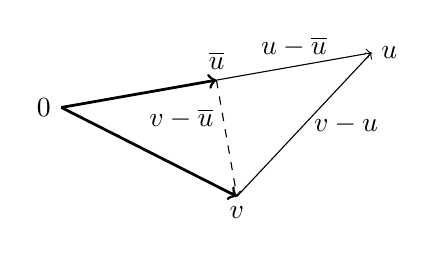
\begin{tikzpicture}[rotate=10]
        \draw[->, line width=1pt] (0,0) node[anchor=east] {0} -- (2,0) node[anchor=south] {$\overline{u}$};
        \draw[->, dashed] (2,0) -- (2,-1.5) node[anchor=north] {$v$};
        \draw[->] (2,-1.5) -- (4,0) node[anchor=west] {$u$};
        \draw[->] (2,0) -- (4,0);
        \draw[->, line width=1pt] (0,0) -- (2,-1.5);
        \draw (3,0)  node[anchor=south] {$u-\overline{u}$};
        \draw (2,-0.5)  node[anchor=east] {$v-\overline{u}$};
        \draw (3,-0.75)  node[anchor=west] {$v-u$};
      \end{tikzpicture}
    \end{image}
    Sei  $u\in U$. Dann gilt
    \begin{align}
      \nonumber
      \nn[v-u]^2 &= \nn[v-\overline{u}+\overline{u} -u]^2 \\ \nonumber
                 &= \nn[v-\overline{u}]^2 +
                   2\underbrace{\scp{v-\overline{u}}{\overbrace{\overline{u}-u}^{~~\in U}}}_{=0}
                   + \nn[u-\overline{u}]^2 \\
                 &= \nn[v-\overline{u}]^2 + \nn[u-\overline{u}]^2
                   \label{IV.3.5}
    \end{align}
    (Dies ist anschaulich der Satz des Pythagoras.)
    Damit ist $\nn[v-u]$ für ein $u\in U$ genau dann minimal, 
    wenn $\nn[u-\overline{u}]$ minimal ist,
    also wenn $u=\overline{u}$.
  \end{enumerate}
\end{proof}


\begin{Satze}
  Der Vektor $\overline{x} \in\R^n$ ist genau dann Lösung
  des linearen Ausgleichsproblems $\min_{x\in\Ren} \nn[b-Ax]_2$,
  falls er die Normalengleichung
  \begin{gather}
    A^TA\overline{x} = A^Tb
    \label{IV.3.6}
  \end{gather}
  erfüllt.
  Insbesondere ist $\overline{x}$ eindeutig,
  falls $A\in \R^{m\times n}$ maximalen Rang $n\leq m$ hat.
\end{Satze}

\begin{proof} Bezeichne
  $V= \R^m, U= R(A) = \left\{Ax \mid x \in\Ren \right\}, b \in\R^m$.
  Nach \eqref{IV.3.3} gilt
  \begin{alignat*}{2}
    &&\nn[b-A\overline{x}]_2 &= \min_{x\in\Ren} \nn[b-Ax]_2 \\
    &\Leftrightarrow \quad & \scp{b-A \overline{x}}{Ax} &= 0 \quad \forall x\in \Ren \\
    &\Leftrightarrow & \scp{A^T(b-A\overline{x})}{x} &= 0 \quad  \forall x\in\Ren \\
    &\Leftrightarrow & A^T(b-A\overline{x}) &= 0 \\
    &\Leftrightarrow & A^TA\overline{x} &= A^Tb
  \end{alignat*}
  Nach dem Projektionssatz \ref{4.3.3} existiert ein eindeutiges
  $\overline{y} = P b$.
  Für dieses $\overline{y}$ ist $\overline{x}\in \Ren $
  mit $\overline{y} = A\overline{x}$ eindeutig bestimmt, 
  falls $A$ injektiv ist, d.h. falls $\Rang(A) = n$. 
\end{proof}

Ähnlich zum Skalarprodukt ist die relative Kondition von $(P,b) $ schlecht, 
falls $b$ fast senkrecht zu $U$ steht.
Die relative Kondition des linearen Ausgleichsproblems
hängt zusätzlich von $\Cond(A)$ ab.


\subsectione{Lösung der Normalgleichung}
Falls $\Rang(A) = n$, ist $A^TA$ spd und das Cholesky-Verfahren ist anwendbar.
Dafür ist
\begin{enumerate}[1.]
\item $A^TA$ zu berechnen:
  \begin{description}
  \item[Aufwand] ca. $\frac{1}{2}n^2m$ Multiplikationen 
  \item[Kondition] häufig schlecht, da $\frac{1}{2}n^2$ Skalarprodukte berechnet werden
  \end{description}
\item die Cholesky-Zerlegung von $A^TA $ durchzuführen:
  \begin{description}
  \item[Aufwand] ca. $\frac{1}{6}n^3$ Multiplikationen 
  \item[Kondition] Für $A\in\R^{m\times n}$ mit $m\geq n$ und
    $\Rang(A)=n$ gilt
    (siehe Übungsaufgabe 19)
    \begin{gather}
      \Cond_2(A^TA) = \Cond_2(A)^2 \label{IV.3.7}
    \end{gather}
  \end{description}
\end{enumerate}
Also überwiegt für $m\gg n$ der Aufwand $A^TA$ zu berechnen.
Die auftretenden Konditionen entsprechen 
i.d.R. nicht dem des Ausgangsproblems.
Damit ist die 
\textbf{Cholesky-Zerlegung\index{Cholesky-Zerlegung} 
  für Normalgleichungen ungeeignet}.


\begin{Satze}
  Sei $A\in \R^{m\times n} $ mit $m\geq n$ und $\Rang(A) = n$,
  sei $b\in\R^m$ und besitze $A$ eine Zerlegung
  \begin{gather*}
    A= Q\begin{pmatrix}R\\0\end{pmatrix}
  \end{gather*}
  mit einer orthogonalen Matrix $Q\in R^{m\times m}$ und 
  einer oberen Dreiecksmatrix $R\in \R^{n\times n}$. 
  Dann ist $R$ invertierbar. 
  Bezeichne 
  \begin{gather}
    \begin{pmatrix} \overline{b}_1 \\ \overline{b}_2\end{pmatrix}
    \coloneqq Q^T\cdot b
    \label{IV.3.9}
  \end{gather}
  dann ist
  \begin{gather}
    \overline{x} = R^{-1} \overline{b}_1 
    \label{IV.3.10}
  \end{gather}
  die Lösung des linearen Ausgleichsproblems und
  \begin{gather*}
    \nn[\overline{b}_2] = \nn[b-A\overline{x}] 
    = \min_{x\in \Ren }\nn[b-Ax]
  \end{gather*}
\end{Satze}

Zur Erinnerung:
$Q \text{ orthogonal} :\Leftrightarrow QQ^T = I
\Leftrightarrow Q^{-1} = Q^T$\\
Weiterhin ist $Q$ längenerhaltend\index{längenerhaltend},
d.h. $\nn[Qv]_2 = \nn[v]_2$, und somit folgt
$\nn[Q]_2 = \nn[Q^{-1}]_2 = 1$ sowie
\begin{gather}
  \Cond_2(Q) = 1
  \label{IV.3.11}
\end{gather}

\begin{proof} $R$ ist invertierbar, da 
  $\Rang(R) = \Rang(Q^{-1}\cdot A) = \Rang(A) = n$.
  Außerdem gilt
  \begin{align*}
    \nn[b-Ax]_2^2 & = \nn[Q\left(Q^Tb-\begin{pmatrix}R\\0\end{pmatrix}x\right)]_2^2 \\
                  &=  \nn[Q^Tb-\begin{pmatrix}Rx\\0\end{pmatrix}]_2^2  \\
                  &\overset{\mathllap{\text{$Q$ längenerhaltend}}}{=}
                    \nn[\overline{b}_1 - Rx]_2^2  + \nn[\overline{b}_2^2]
  \end{align*}
  wird minimal für $R\overline{x} = \overline{b}_1$.
\end{proof}

Da $Q$ längenerhaltend ist, folgt mit \ref{3.2.13}b)
($\Cond_A \coloneqq \frac{\max \nn[Ax]}{\min \nn[Ax]}$)
sofort
\begin{gather*}
  \Cond_2(A) = \Cond_2(R)
\end{gather*}
Die auftretende Kondition entspricht also der des Ausgleichsproblems.


% \subsectione{Bemerkung}
\begin{Beme}
  Sei $A\in \Renn$ invertierbar und habe ein QR-Zerlegung, d.h. es existiert
  eine orthogonale Matrix $Q$ und eine obere Dreiecksmatrix $R$, so dass:
  \begin{gather*}
    A= Q\cdot R
  \end{gather*}
  Dann kann das Gleichungssystem $Ax=b$ wie folgt gelöst werden:
  \begin{enumerate}[1.]
  \item Setze $z=Q^Tb$, was Kondition 1 hat.
  \item Löse durch Rückwärtssubstitution $Rx=z$.
  \end{enumerate}
\end{Beme}


% -------------------------------------------------------------

\sectione{Orthogonalisierungsverfahren}\index{Orthogonalisierung}
\marginpar{12.11.2014}
Konstruiere eine QR-Zerlegung
\begin{gather}
  A= Q\cdot \begin{pmatrix} R\\0 \end{pmatrix}
  \label{IV.4.1}
\end{gather}
durch einen Eliminationsprozess:
\begin{gather}
  A \longrightarrow Q^{(1)}A 
  \longrightarrow Q^{(2)} Q^{(1)}A 
  \longrightarrow Q^{(p)}\dotsm Q^{(1)}A
  = \begin{pmatrix} R\\0 \end{pmatrix}
  \label{IV.4.2}
\end{gather}
mit orthogonalen Matrizen $Q^{(i)}$.
Dann gilt
\begin{gather}
  Q= Q^{(1)T}\dotsm {Q^{(p)T}}
  \label{IV.4.3}
\end{gather}
Dies ist im Gegensatz zur LR-Zerlegung aufgrund von $\Cond(Q^{(i)})= 1$ immer stabil.

Für $Q\in\R^{2\times 2}$ gibt es zwei mögliche Anschauungen, nämlich:
\begin{enumerate}[a)]
\item Drehung ~~~
  \begin{tikzpicture}
    \coordinate (a) at (30:2cm);
    \coordinate (b) at (2,0);
    \coordinate (z) at (0,0);
    \draw [->] (0,0) -- (a) node[anchor=west] {a};
    \draw [->] (0,0) -- (b);
    \draw[->] (b) -- (0,0) -- (a)
    pic [draw=black,angle radius=13mm, "$\theta$"] {angle = b--z--a};
  \end{tikzpicture}\label{im4.4(1)}
\item Spiegelung ~~~
  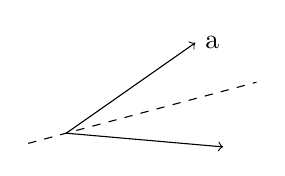
\begin{tikzpicture}[rotate=15]
    \coordinate (a) at (20:2cm);
    \coordinate (b) at (-20:2cm);
    \coordinate (z) at (0,0);
    \draw[dashed] (-0.5, 0) -- (2.5, 0);
    \draw[->] (z) -- (a)  node[anchor=west] {a};
    \draw[->] (z) -- (b);
  \end{tikzpicture}\label{im4.4(2)}
\end{enumerate}

\extrasection{a)}{Givens-Rotation}
Es wird eine Drehung auf den 1. Einheitsvektor durchgeführt:
\begin{image}{Drehung auf den Einheitsvektor}
  \begin{tikzpicture}
    \coordinate (a) at (30:2cm);
    \coordinate (b) at (2,0);
    \coordinate (z) at (0,0);
    \draw [->] (0,0) -- (a) node[anchor=west] {$a$};
    \draw [->] (0,0) -- (b) node[anchor=west] {$\alpha e_1$};
    \draw (a) -- (0,0) -- (b)
    pic [draw=black,angle radius=9mm, "$\theta$"] {angle = b--z--a};
    \draw[->, dashed] (30:18mm) arc [start angle=30, end angle=0, radius=18mm];
  \end{tikzpicture}
  \label{im4.4.a}
\end{image}
\begin{gather*}
  a=\begin{pmatrix}a_1 \\ a_2\end{pmatrix} \longrightarrow \begin{pmatrix}\alpha \\ 0 \end{pmatrix}
  = \alpha e_1
\end{gather*}
d.h. Elimination von $a_2$ mit $\nn[\alpha e_1]_2 = \nn[a]_2$.
Also gilt $\alpha=\pm \nn[a]_2$.
Drehungen werden beschrieben durch
\begin{gather*}
  Q = \begin{pmatrix}
    cos(\theta) & sin(\theta)\\
    -sin(\theta) & cos(\theta)
  \end{pmatrix}
  \eqqcolon \begin{pmatrix}
    c & s\\
    -s & c
  \end{pmatrix}\qquad \theta \in[0,2\pi)
\end{gather*}
und es muss gelten $Qa = \begin{pmatrix}\alpha\\0\end{pmatrix}$.
Hiermit folgt für $\nn[a]= 0$, dass $c=1, s=0$,
und für $\nn[a]\neq 0$, dass
$c=\frac{a_1}{\alpha},  s= \frac{a_2}{\alpha}$ mit
\begin{gather}
  \alpha = \pm \sqrt{a_1^2+a_2^2}
  \label{IV.4.4}
\end{gather}
Im Folgenden wird dies kurz mit $[c,s] = \Givens(a_1, a_2)$ bezeichnet.
Als \textbf{Givens-Rotation}\index{Givens-Rotation} wird eine Matrix der Form
\begin{gather}
  \Omega _{k,l} = \begin{pmatrix}
    1 &&&&&&&&& \\
    & \ddots\\
    && 1\\
    &&& \mathbf{c} &&&& \mathbf{s} \\
    &&&& 1\\
    &&&&& \ddots \\
    &&&&&& 1\\
    &&& -\mathbf{s} &&&& \mathbf{c} \\
    &&&&&&&& \ddots \\
    &&&&&&&&& 1\\
  \end{pmatrix}
  \begin{array}{l}
    \\   \leftarrow \text{$k$-te Zeile}
    \\ \\ \\ \\ \leftarrow \text{$l$-te Zeile}
  \end{array}
  \label{IV.4.5}
\end{gather}
mit $c^2+s^2=1$ und $k<l$ bezeichnet.
Es folgt
\begin{align*}
  \Omega_{kl} A &= \widetilde{A} \quad \text{mit} \\
  \widetilde{a}_{ij}  &= a_{ij} \quad \text{ für } i\neq k,l \\
  \widetilde{a}_{kj} & = ca_{kj}+sa_{lj} \\
  \widetilde{a}_{lj} & = -sa_{kj} + ca_{lj}
\end{align*}
Demnach werden nur die $k$-te und $l$-te Zeile werden verändert. \\
Falls nun $[c,s] = \Givens(x_k, x_l)$ gilt
\begin{gather}
  \Omega_{k,l}\cdot x = \begin{pmatrix}
    x_1 \\ \vdots\\x_{k-1} \\\alpha \\ x_{k+1}
    \\\vdots \\
    x_{l-1} \\ 0 \\x_{l+1} \\\vdots \\x_n
  \end{pmatrix}
  \qquad
  \quad \text{mit~~}
  \alpha = \pm \nn[  \begin{pmatrix} x_k \\ x_l\end{pmatrix}]_2
  \label{IV.4.6}
\end{gather}
d.h. eine Givens-Rotation erzeugt eine Null.\\
Da nun
\begin{gather*}
  \R^{m\times n}\ni \begin{pmatrix}
    * & * &* & \cdots   \\
    0 & * &     \\
    0 & 0 & \ddots \\
    \vdots \\
    0 & 0 & 0 & \cdots & *		
  \end{pmatrix}
  = \begin{pmatrix} R\\0\end{pmatrix}
\end{gather*}
gilt, sind $p=\sum_{j=1}^{n}(m-j)$ Givens-Rotationen nötig,
um eine QR-Zerlegung nach \eqref{IV.4.1} zu erzeugen.
Und eine Rotation, welche $a_{ij} $ auf 0 setzt, ist durch zugehörige 
$(c_{ij}, s_{ij}) $ gegeben.

Für eine 3x4-Matrix sieht das Verfahren folgendermaßen aus:

\begin{align*}
  A= &
       \left(\begin{array}{lcc}
               *~ &&\\
               * &* \\
               * \rcurvearrownw \\ * \lcurvearrowsw
             \end{array}\right)
  \quad \overset{\Omega_{3,4}}{\longrightarrow} \quad
  \left(\begin{array}{lcc}
          *~ &&\\
          * \rcurvearrownw & *\\
          * \lcurvearrowsw \\
          0
        \end{array}\right)
  \quad \overset{\Omega_{1,2}}{\longrightarrow} \quad
  \left(\begin{array}{lcc}
          * \rcurvearrownw\\
          * \lcurvearrowsw & *& \\
          0 \\
          0
        \end{array}\right)\\
  \quad \overset{\Omega_{2,3}}{\longrightarrow} \quad
     &\left(\begin{array}{lcc}
              *~~ \\
              0 && * \\
              0 \\
              0
            \end{array}\right)
  \quad \overset{\Omega_{3,4}}{\longrightarrow} \quad	
  \left(\begin{array}{clc}
          * & *\\
          0 & *  \rcurvearrownw  & * \\
          0 & * \lcurvearrowsw \\
          0 & 0
        \end{array}\right)
              \quad \overset{\Omega_{2,3}}{\longrightarrow} \quad	
              \left(\begin{array}{ccl}
                      * & *  & * \\
                      0 & *  & * \\ 
                      0 & 0 & * \rcurvearrownw\\
                      0 & 0 & *  \lcurvearrowsw 
                    \end{array}\right) \\
  \quad \overset{\Omega_{3,4}}{\longrightarrow} \quad	
     & \left(\begin{array}{ccc}
               * & *  & *  \\
               0 & *  & * \\ 
               0 & 0 & * \\
               0 & 0 & 0
             \end{array}\right)
                       = \begin{pmatrix}
                         R \\ 0 
                       \end{pmatrix}
\end{align*}

Es ergibt sich:

\subsectione{Givens-QR-Algorithmus} \index{Givens-QR-Algorithmus}

\begin{pseudocode}{0.7\linewidth}
  \textbf{for} $j=1, \dotsc , n$ \\
  |~	\>	\textbf{for} $i=m, m-1, \dotsc , j+1$ \\
  |~	\>		|~	\>\% \textit{setze $a_{ij}$ auf 0} \\
  |~	\>		|~	\>$[c,s] = \Givens(a_{i-1,j}, \dotsc, a_{ij}) $\\
  |~	\>		|~	\>speichere $c$ und $s$ für $a_{ij}$ \\
  |~	\>		|~	\>$A(i-1:j, j:h) = \left(
    \begin{smallmatrix}c & s\\-s & c \end{smallmatrix}
  \right) * A(i-1:j, j:n)$ \\
  |~	\> \textbf{end}\\
  \textbf{end}							
\end{pseudocode}


\begin{Beme}~
  \begin{enumerate}[a)]
  \item $A(i-1 : i, 1 : j-1) = 0$ und ist daher nicht zu berechnen oder
    zu speichern. Der Speicherplatz kann für die Speicherung der
    Givensrotationen benutzt werden.
  \item  $R$ steht anschließend in $A$.
  \item Die Bestimmung der Länge $|\alpha|$ wird so ausgeführt, dass over-
    oder underflow vermieden wird. Weiterhin wird das Vorzeichen
    von $c$ oder $s$ festgelegt, so dass aufgrund von $c^2+s^2=1$ nur
    ein Wert $\rho$ gespeichert werden muss. Hiermit wird auch das
    Vorzeichen von $\alpha$ festgelegt:
    \begin{description}
    \item[$a_2=0$:] Setze $c=1, s=0, \alpha = a_1$, merke $\rho=1$.
    \item[$|a_2|>|a_1|$:] Setze 
      $\tau= \frac{a_1}{a_2}, s=\frac{1}{\sqrt{1+\tau^2}}, 
      c=s\cdot\tau, \alpha =a_2\sqrt{1+\tau^2}$, 
      merke $\rho=\frac{c}{2}$.
    \item[$|a_1|\geq|a_2|$:] Setze 
      $\tau= \frac{a_2}{a_1}, c=\frac{1}{\sqrt{1+\tau^2}}, 
      s=c\cdot\tau, \alpha =a_1\sqrt{1+\tau^2}$, 
      merke $\rho=\frac{2}{s}$.
    \end{description}
  \item Aufgrund von c) muss nur $\rho$ gespeichert werden:
    \begin{description}
    \item[$\rho=1$:] Setze $c=1, s=0$.
    \item[$|\rho|<1$:] Setze $c=2\rho , s= \sqrt{1-c^2}$.
    \item[$|\rho|>1$:] Setze $s=\frac{2}{\rho}, c=\sqrt{1-s^2}$.
    \end{description}
  \end{enumerate}
  Hiermit können alle notwendigen Givens-Rotationen als untere
  Dreiecksmatrix zusammen mit $R$ in $A$ gespeichert werden.
\end{Beme}


\subsectione{Aufand des Givens-QR-Algorithmus}
\begin{enumerate}[a)]
\item $m\approx n$\\ $\longrightarrow $  ca. $\frac{4}{3}n^3$ Multiplikationen
  und $\frac{1}{2}n^2$ Quadratwurzeln nötig \\
  Die Givens-QR-Zerlegung ist somit ungefähr viermal so aufwändig
  wie die Gauß-Elimination, dafür jedoch stabil.
\item $m\gg n$\\ $\longrightarrow $ ca. $2n^2m$ Multiplikationen und 
  $mn$ Quadratwurzeln nötig \\
  Das Verfahren ist daher zwei- bis viermal so aufwändig wie das
  Cholesky-Verfahren für die Normalgleichungen, aber stabil.
\item Bei Hessenberg-Matrizen, d.h. Matrizen mit der Gestalt
  \begin{gather}
    A= \begin{pmatrix}
      * & \cdots&& * \\
      *&* \\
      &\ddots& \ddots \\
      \\
      0 &&& * 
    \end{pmatrix}
    \label{IV.4.7} \, ,
  \end{gather}
  also $a_{ik} = 0 \forall i<k+1$,
  sind nur $(n-1)$ Givens-Rotationen auszuführen.
  Diese Matrizen tauchen z.B. bei Eigenwertberechnungen auf
  und sind dort ein wichtiger Bestandteil der Verfahren.
\end{enumerate}


\extrasection{b)}{Householder-Reflexion}

Es sei $H$ eine Hyperebene im $\R^m$ und zusätzlich ein Vektor
$a\in\R^m$ gegeben.

\begin{image}{\copyright~ Householder-Reflexion}
  \begin{tikzpicture}[rotate=30, >=triangle 45,scale=4]
    \draw (0,0) -- (2,0) node[below] {$H$};
    \draw[->] (0.5,0) -- (1,0.7);
    \draw[->] (0.5,0) -- (1,-0.7);
    \draw (1,0.7) -- (1,-0.7);
    \draw[anchor=east] (0.8,0.4) node {$a\in \R^m$};
    \draw[anchor=east] (0.8,-0.5) node {$\alpha e_1$};
    \draw (0.9,0) arc (180:90:1mm);
    \draw[fill=black] (0.96,0.04) circle (0.05mm);
  \end{tikzpicture}
\end{image}

Gesucht ist nun die Reflexion $Q$, so dass
\begin{gather*}
  Qa = \alpha e_1 
  = \begin{pmatrix} \alpha \\ 0\\\vdots\\0\end{pmatrix}
  \qquad \text{mit } \alpha = \pm \nn[a]
\end{gather*}
wobei \begin{gather}
  v=a-\alpha e_1 
  \label{IV.4.8}
\end{gather}
gegeben ist, welches senkrecht zu $H$ steht.
Damit Stellenauslöschungen in $v$, d.h. in $v_1$, vermieden werden,
wähle ein entsprechendes Vorzeichen für $\alpha$, also 
\begin{gather}
  \alpha = -\Sign(a_1)\nn[a]_2 
  \label{IV.4.9}
\end{gather}
Die zugehörige Reflexion $Q$ ist  gegeben durch
\begin{image}{\copyright}
  \begin{tikzpicture}[line cap=round,line join=round,>=triangle 45,x=1.0cm,y=1.0cm]
    \clip(0.7,1) rectangle (6,5);
    \draw [shift={(4.32,3.49)}] (0,0) -- (36.87:0.6) arc 	(36.87:126.87:0.6) -- cycle;
    \draw [shift={(1.53,2.76)}] (0,0) -- (-53.13:0.6) arc (-53.13:36.87:0.6) -- cycle;
    \draw [domain=0.7:6] plot(\x,{(--1--3*\x)/4});
    \draw (5.26,4.38) node[anchor=north west] {$$H$$};
    \draw [->] (2.18,1.89) -- (0.84,3.68);
    \draw [->] (2.18,1.89) -- (3.66,4.36);
    \draw [->] (2.18,1.89) -- node[anchor=north east] {$w$} (1.53,2.76);
    \draw [->,dash pattern=on 2pt off 2pt] (2.18,1.89) -- node[anchor=north] {$Qx$} (4.97,2.61);
    \draw [->] (3.66,4.36) -- (4.97,2.61);
    \fill(4.37,3.84) circle (0.02);
    \draw [dash pattern=on 2pt off 2pt] (1.53,2.76)-- (3.66,4.36);
    \fill(1.88,2.71) circle (0.02);
    
    \draw (1.26,3.46) node {$v$};
    \draw (4.3,3.1) node {$2w$};
  \end{tikzpicture}
\end{image}		

wobei
\begin{align}
  \nonumber
  w &= \scp{\frac{v}{\nn[v]}}{x} \cdot \frac{v}{\nn[v]} \\ %\nonumber
  Qx &= x-2w = x-2\frac{v^Tx}{v^Tv}v 
       = (I-2\frac{vv^T}{v^Tv})x 
       \label{IV.4.10}\\
  Q  &= I-2\frac{vv^T}{v^Tv}&& vv^T \in \Renn,\,\, v^Tv\in\R
                               \label{IV.4.11}
\end{align}
und heißt \textbf{Householder Reflexion} \index{Householder Reflexion}
(wurde  1958 von Householder eingeführt).  \\
Für die spezielle Wahl \eqref{IV.4.8} mit \eqref{IV.4.9} vom Vektor $v$ folgt
\begin{align}\nonumber
  vv^T = \nn[v]^2 &= \nn[a]^2 - 2\alpha\scp{a}{e_1} + \alpha^2 \\ \nonumber
                  &= -2\alpha(a_1-\alpha) \\
                  & = -2\alpha v
                    \label{IV.4.12}
\end{align}


\begin{Beme}
  \label{4.4.4}~
  \begin{enumerate}[a)]
  \item Q ist symmetrisch
  \item Q ist orthogonal
  \item Q ist involutorisch, d.h. $Q^2 = I$ ~~(bzw. gilt $Q^{-1}= Q^T=Q$)
  \end{enumerate}
  Die Householder Reflexion setzt nicht nur eine Null,
  sondern im Vektor gleich alle gewünschten Nullen
  \begin{align*}
    \text{\textbf{Rotation: }}&
                                \quad \begin{pmatrix} * \\ * \\ *	\end{pmatrix}
    \rightarrow \begin{pmatrix} * \\ * \\0	\end{pmatrix}
    \rightarrow \begin{pmatrix} * \\0\\0	\end{pmatrix} \\
    \text{\textbf{Reflexion: }}&
                                 \quad \begin{pmatrix} * \\ * \\ *	\end{pmatrix}
    \rightarrow \begin{pmatrix} *\\0\\0	\end{pmatrix}
  \end{align*}
  Um die erste Spalte in $A$ auf die gewünschte Gestalt zu bringen,
  bestimme $Q^{(1)}$ wie oben, indem die erste Spalte als $a$ gewählt wird:
  \begin{gather*}
    A\rightarrow A^{(1)} = Q^{(1)} A =
    \begin{pmatrix}
      \alpha^{(1)} \\
      0 &*&~~\\
      \vdots \\
      0
    \end{pmatrix}
  \end{gather*}
  In der $k$-ten Spalte sollen nun die $(k-1)$-ten Zeilen und die $(k-1)$-ten Spalten
  bleiben und die Restmatrix verändert werden.
  
  \begin{align*}
    A^{(k-1)} &=
                \begin{pmatrix}
                  *  &&&&&\\
                  &\ddots &&&& * \\
                  &&*&&\_&\_&\_ \\
                  &&0&|&\\
                  &0&\vdots&| &&T^{(k-1)}\\
                  &&\vdots&  |\\
                  &&0&  |
                \end{pmatrix}
                       \begin{array}{l}
                         \\
                         \shortleftarrow (k-1) \text{-te Zeile} \\
                         \\\\\\\\
                       \end{array}\\
              &\phantom{= \, (} \begin{array}{ccl}
                                  ~&~&~ \uparrow (k-1)\text{-te Spalte}
                                \end{array}
  \end{align*}
  
  Setze also
  \begin{gather}
    Q^{(k)} = \begin{pmatrix}
      I_{k-1} & 0 \\
      0 & \overline{Q}^{(k)}
      \label{IV.4.13}
    \end{pmatrix}\, ,
  \end{gather}
  wobei $\overline{Q}^{(k)} $ durch die erste Spalte von $T^{(k)}$, d.h.
  \begin{gather}
    a= (a_{i,k}^{k-1})_{i=k,\dotsc, m} \subset \R^{m+1-k}
    \label{IV.4.14}
  \end{gather}
  bestimmt wird. Dann gilt
  \begin{gather*}
    Q^{(k)}A^{(k-1)} =
    \begin{pmatrix}
      *  &&&&&\\
      &\ddots &&&& * \\
      &&*&&\_&\_&\_&\_ \\
      &&0&|&* \\
      &0&\vdots&|&0&* \\
      &&\vdots&  |&\vdots &&\ddots\\
      &&0&  |&0&&&*
    \end{pmatrix}
  \end{gather*}
  Nach insgesamt 
  \begin{gather}
    p=\min (m-1, n)
    \label{IV.4.15}
  \end{gather}
  Schritten erhalten wir für $A\in \R^{m\times n}$
  \begin{gather}
    Q^TA = Q^{(p)}\dotsm Q^{(1)}A 
    = \begin{pmatrix} R\\0\end{pmatrix}\, ,
  \end{gather}
  wobei Bemerkung \ref{4.4.4} auch für 
  $Q^T= Q^{(p)}\dotsm Q^{(1)} $ und somit auch für
  \begin{gather}
    Q = Q^{(1)}\dotsm Q^{(p)}
    \label{IV.4.16}
  \end{gather}
  gilt.
\end{Beme}



% ----------------------------------------------------------------

\subsectione{Speicherung}
\marginpar{17.11.2014}
Gespeichert werden müssen die obere Dreiecksmatrix $R$ und die 
\textbf{Householdervektoren} \index{Householdervektoren}
$v^{(i)}\in \R^{m+1-i}$.
Die Diagonalelemente von $R$ sind $r_{ii} = \alpha^{(i)}$. \\
Folgende Speicheraufteilung ist möglich:
\begin{gather*}
  A \longrightarrow \left(
    \begin{array}{rrrrr}
      |&&& R \\
      |&| \\
      v^{(1)}| & v^{(2)}|&\ddots ~~\\
      | &|&\phantom{v^{(i)}}|& v^{(p)}			
    \end{array}
  \right)
  \quad \text{und} \quad 
  \begin{pmatrix}
    \alpha^{(1)} \\ \vdots \\ \\ \alpha^{(p)}
  \end{pmatrix}
\end{gather*}
Wohlgemerkt kann so auch $A\in \R^{m\times n}$ mit $m<n$ bearbeitet werden,
dann wird $A$ zu:

\imagemissing{Zerlegung einer $m\times n$-Matrix für $m<n$}\label{im4.4.5}

Falls zusätzlich $v^{(i)}$ so normiert ist,
dass $v_1^{(i)} = 1$ ist, braucht diese Komponente nicht gespeichert werden 
und $R$ kann komplett in $A$ gespeichert werden.


\subsectione{Householder QR-Algorithmus}
\begin{pseudocode}{\linewidth}
  \textbf{for} $j = 1,\dotsc, \min(m - 1, n)$ \\
  |	\>	// berechne $\alpha$ für $a = A(j : m, j)$ \\
  |	\>	$\alpha(j) = -\Sign(A(j, j))\sqrt{A(j:m, j)^T A(j:m, j)}$ \>\>\>\> siehe \eqref{IV.4.9}\\
  |	\>  // berechne $A(j:m,j)=v=a-\alpha e_1$ \\
  |	\>	$A(j,j)=A(j,j)-\alpha(j)$ \>\>\>\> siehe \eqref{IV.4.8}\\
  |	\> // berechne $-\scp{v}{v} = \alpha(a_1 - \alpha) = \alpha v_1$ \\
  |	\> $\beta = \alpha(j)A(j, j)$\>\>\>\> siehe \eqref{IV.4.12}\\
  |	\> // berechne $\overline{Q}^{(j)}T^{(j)}$ 
  aber nicht mehr die erste Spalte, welche $\alpha(j)e_1$ ist\\
  |	\> \textbf{for} $l = j + 1 : n$\\
  |		\>\> // setze $v_x = -2{(v^Tx)}{(v^Tv)}^{-1}$\\
  |		\>\> $v_x = A(j : m, j)^TA(j:m,l)\cdot \frac{1}{\beta}$ \>\>\>siehe \eqref{IV.4.10}\\
  |		\>\> // berechne  $\overline{Q}^{(j)}x=x+v_x\cdot v$\\
  |		\>\> $A(j:m,l) = A(j:m,l)+v_xA(j:m,l)$ \>\>\> siehe \eqref{IV.4.10}\\
  |	\>\textbf{end}\\
  \textbf{end}
\end{pseudocode}


\subsectione{Berechnung von $Q^Tb$}
Zur Lösung eines Gleichungssystems oder eines linearen Ausgleichsproblems
muss noch $Q^Tb=Q^{(p)}\dotsm Q^{(1)}$ berechnet werden.

\begin{pseudocode}{0.7\linewidth}
  \textbf{for} $j=1,\dotsc, \min\{m-1,n\}$\\
  |	\> // beachte \eqref{IV.4.13}, also $b(1:j-1)$ bleibt gleich\\
  |	\> // setze $v_x=-2(v^Tb)(v^Tv)^{-1}$\\
  |	\> $v_x=\big(A(j:m,j)^Tb(j:m)\big)\cdot \big(\alpha(j)A(j,j)\big)^{-1}$ \\
  |	\> // berechne $\overline{Q}^{(j)} b=b+v_xv$\\
  |	\> $b(j:m) = b(j:m)+v_xA(j:m,j)$\\
  \textbf{end}
\end{pseudocode}


\subsectione{Aufwand für den Householder-QR-Algorithmus}
\begin{enumerate}[a)]
\item Falls $m\approx n$ sind ungefähr $\frac{2}{3}n^3$ Multiplikationen notwendig
  und ist somit ungefähr doppelt so teuer wie die LR-Zerlegung, ist aber stabil.
\item Falls $m\gg n$ sind ungefähr $2mn^2$ Multiplikationen notwendig.
  Der Aufwand ist daher ungefähr so hoch wie beim Cholesky-Verfahren für Normalgleichungen,
  aber stabil.
\end{enumerate}

%%% Local Variables:
%%% mode: latex
%%% TeX-master: "../numerik_script"
%%% End:
